\documentclass[a4paper, 12pt]{article}

% Добавляем новые пакеты
\usepackage[english, russian]{babel}    % Пакет для поддержки русского языка
\usepackage[T1, T2A]{fontenc}           % Загружаем пакет с поддержкой кирилицы
\usepackage[utf8]{inputenc}             % Загружаем пакет с поддержкой кодировки файла и символов
\usepackage{ragged2e}                   % Загружаем пакет для выравнивания текста
\usepackage{graphicx}                   % Загружаем пакет для добавления различной графики (pdf, jpg, png)
\usepackage{import}                     % Загружаем пакет для продвинутого импорта, в частности изображений pdf_tex из графического редактора inkscape (\import{<path to file>}{<filename>.pdf_tex})
\usepackage{subcaption}                 % Пакет для поддержки сетки из фигур, например в две колонки или матрицей
\usepackage{float}                      % Пакет для улучшенного размещения изображенией (ниже используется опция H в команде \begin{figure}[H])
\usepackage{geometry}                   % Пакет для управления отступами на странице (см. далее вызываем \geometry)
\usepackage{amsmath}                    % Добавляем крутую поддержку математики, в частности /align
\usepackage{amsfonts}                   % Пкет с мтематическими шрифтами вроде \mathbb и др.
\usepackage{tabu}                       % Пакет с прокаченными таблицами
\usepackage{booktabs}                   % Крутые вертикальные разделители
\usepackage[dvipsnames]{xcolor}         % Рассширенная поддержка цветов
\usepackage[colorlinks]{hyperref}
\usepackage{indentfirst}                % Пакет, чтобы починить красную строку
\usepackage{listings}                   % Поддержка листингов, оформления кода программы
\usepackage{src/vpdtitle}               % Титульный лист (смотри файл vpdtitle.sty)

\usepackage{titletoc}
\dottedcontents{section}[2.3em]{}{2.3em}{6pt}
\dottedcontents{subsection}[2.3em]{}{2.3em}{6pt}
\dottedcontents{subsubsection}[2.3em]{}{2.3em}{6pt}

% Устанавливает отступы на странице
\geometry{left=2cm, right=2cm, bottom=2cm, top=2cm}

% Настараиваем красивые цвета для ссылок на формулы, фигуры (изображения) и другие элементы.
\hypersetup{
    linkcolor=blue,
    filecolor=magenta,
    urlcolor=cyan
}

% Настраиваем супер красивые листинги с попомщью пакетов listings и xcolor
\definecolor{codegreen}{rgb}{0,0.6,0}
\definecolor{codegray}{rgb}{0.5,0.5,0.5}
\definecolor{codepurple}{rgb}{0.58,0,0.82}
\definecolor{backcolour}{rgb}{0.95,0.95,0.92}

\lstdefinestyle{codestyle}{
    backgroundcolor=\color{backcolour},
    commentstyle=\color{codegreen},
    keywordstyle=\color{magenta},
    numberstyle=\tiny\color{codegray},
    stringstyle=\color{codepurple},
    basicstyle=\ttfamily\footnotesize,
    breakatwhitespace=false,
    breaklines=true,
    captionpos=b,
    keepspaces=true,
    numbers=left,
    numbersep=5pt,
    showspaces=false,
    showstringspaces=false,
    showtabs=false,
    tabsize=2
}

\lstset{style=codestyle}
\lstset{extendedchars=\true}

%%%%%%%%%%%%%%%%%%%%%%%%%%%%%%%%%%%%%%%%%%%%%%%%
%% Заполнение титульного листа
%%%%%%%%%%%%%%%%%%%%%%%%%%%%%%%%%%%%%%%%%%%%%%%%
\title{
Жёсткая фильтрация
}

% Тут укажите автора
\author{Иван М. Бакланов}
\affil{465112, ibaklanov@niuitmo.ru}

\author{Владимир В. Ананичев}
\affil{464994, vandmitrievic@mail.ru}
% Впишите данные о том, кто будет проверять работу
\supervisor{Артем В. Пашенко}

% Краткое описание того, что сделали в работе
\abstract{
Работа посвящена фильтрации сигналов при помощи рядов Фурье.
}

% Подберите 3-5 ключевых слова, отличающих эту работу от всех остальных
\keywords{
    Python, Fourier series, Filtration
}

\date{\today}







%%%%%%%%%%%%%%%%%%%%%%%%%%%%%%%%%%%%%%%%%%%%%%%%
% Начала всего-всего текста. Здесь идет сам документ, все пишется именно сюда
%%%%%%%%%%%%%%%%%%%%%%%%%%%%%%%%%%%%%%%%%%%%%%%%
\begin{document}

\maketitle

\tableofcontents

\newpage


\section{Жёсткие фильтры}
\subsection{Постановка задачи}

Зададимся следующей функцией
\[
g(t) = \begin{cases}
    3, \quad t \in [-\pi, \pi] \\
    0, \quad t \notin [-\pi, \pi] \\
\end{cases}
\]

\begin{figure}[H]
    \centering
    
\includegraphics[width=1.0\linewidth]{images/function_g.png}
    \caption{Исходная функция}
    \label{fig:func_init}
\end{figure}

Зашумим данную функцию следующим образом
\[
u(t) = g(t) + \xi(t) +  0.8\cdot sin(20t)
\]
Где
\[
\xi(t) = 2*rand() - 1
\]

\begin{figure}[H]
    \centering
    
\includegraphics[width=1.0\linewidth]{images/noise_g.png}
    \caption{Зашумлённая функция}
    \label{fig:noise}
\end{figure}

Получим Фурье-образ зашумлённой функции

\begin{figure}[H]
    \centering
    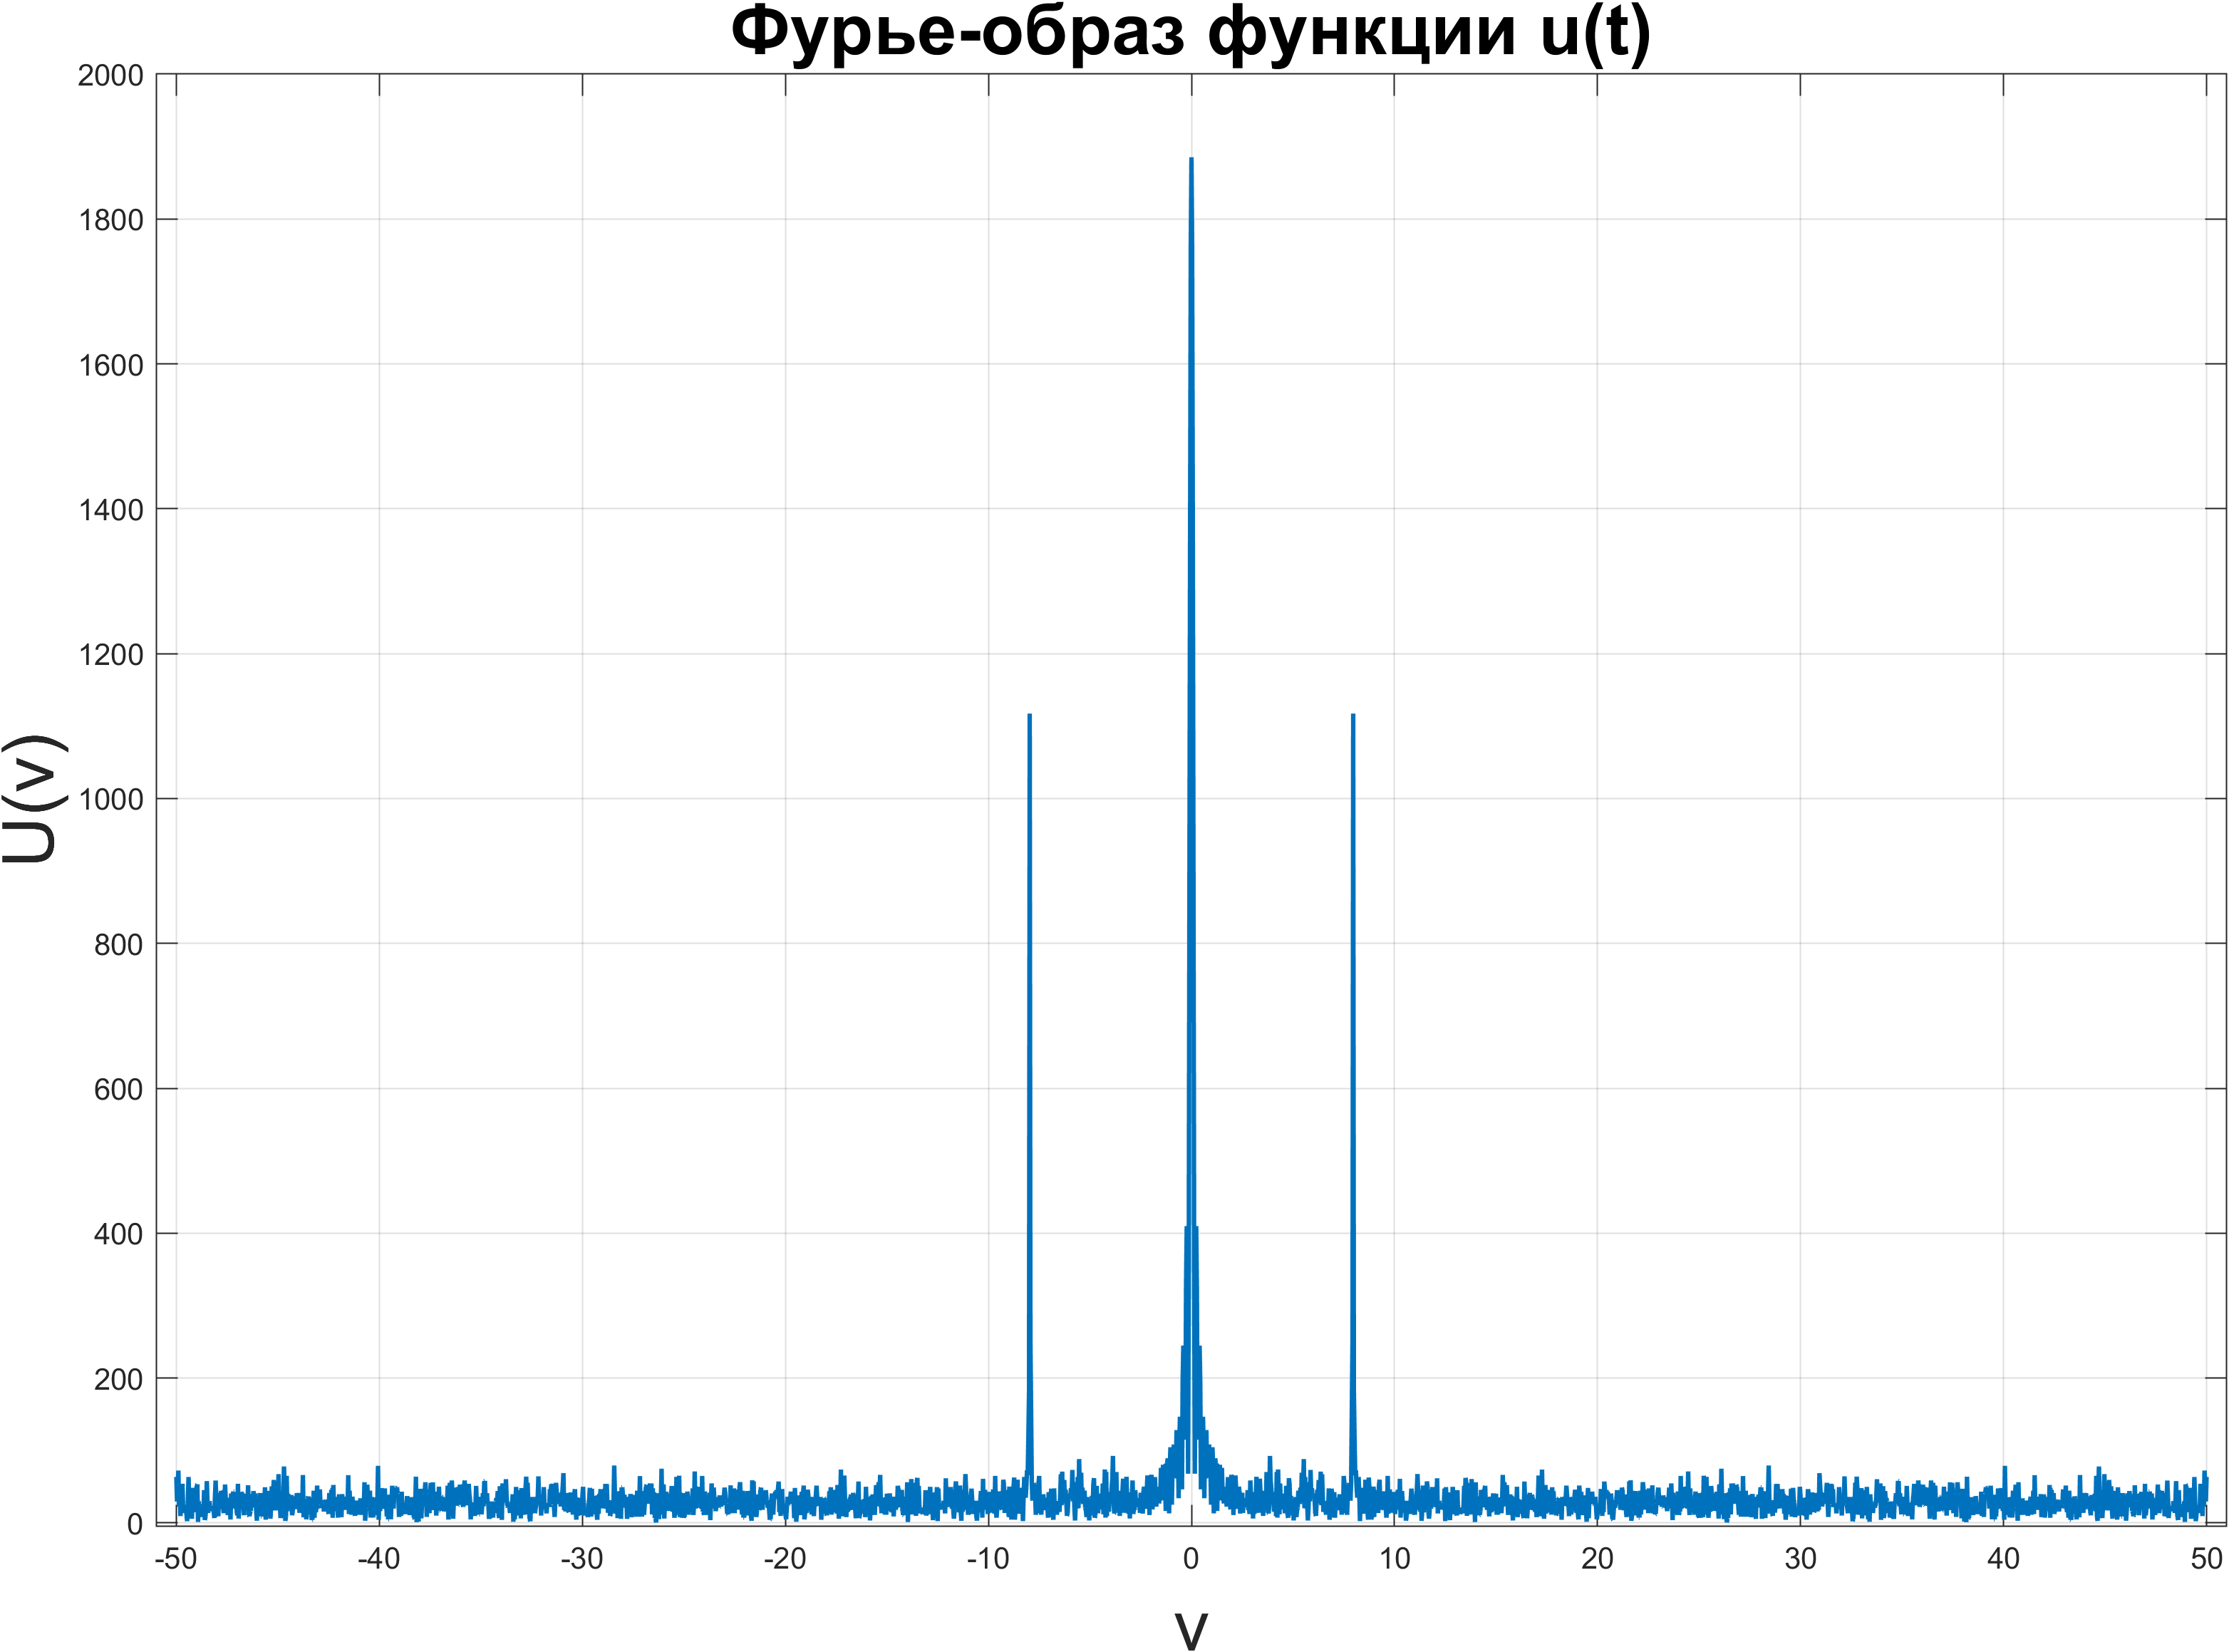
\includegraphics[width=1.0\linewidth]{images/im_noise.png}
    \caption{Зашумлённая функция}
    \label{fig:noise}
\end{figure}

\subsection{Фильтр высоких частот}

Зададимся следующим фильтром


\newpage
\section{Фильтрация звука}

Прослушав аудиофайл с гугл-диска, было очевидно, что шумы, которые присутствуют на записи - низкие частоты, поэтому изначально был применён фильтр высоких частот(ФВЧ). Но на отфильтрованной записи проявились небольшие высокие шумы, поэтому в финальном варианте применён режекторный полосовой фильтр(РПФ).


\begin{figure}[H]
    \centering
    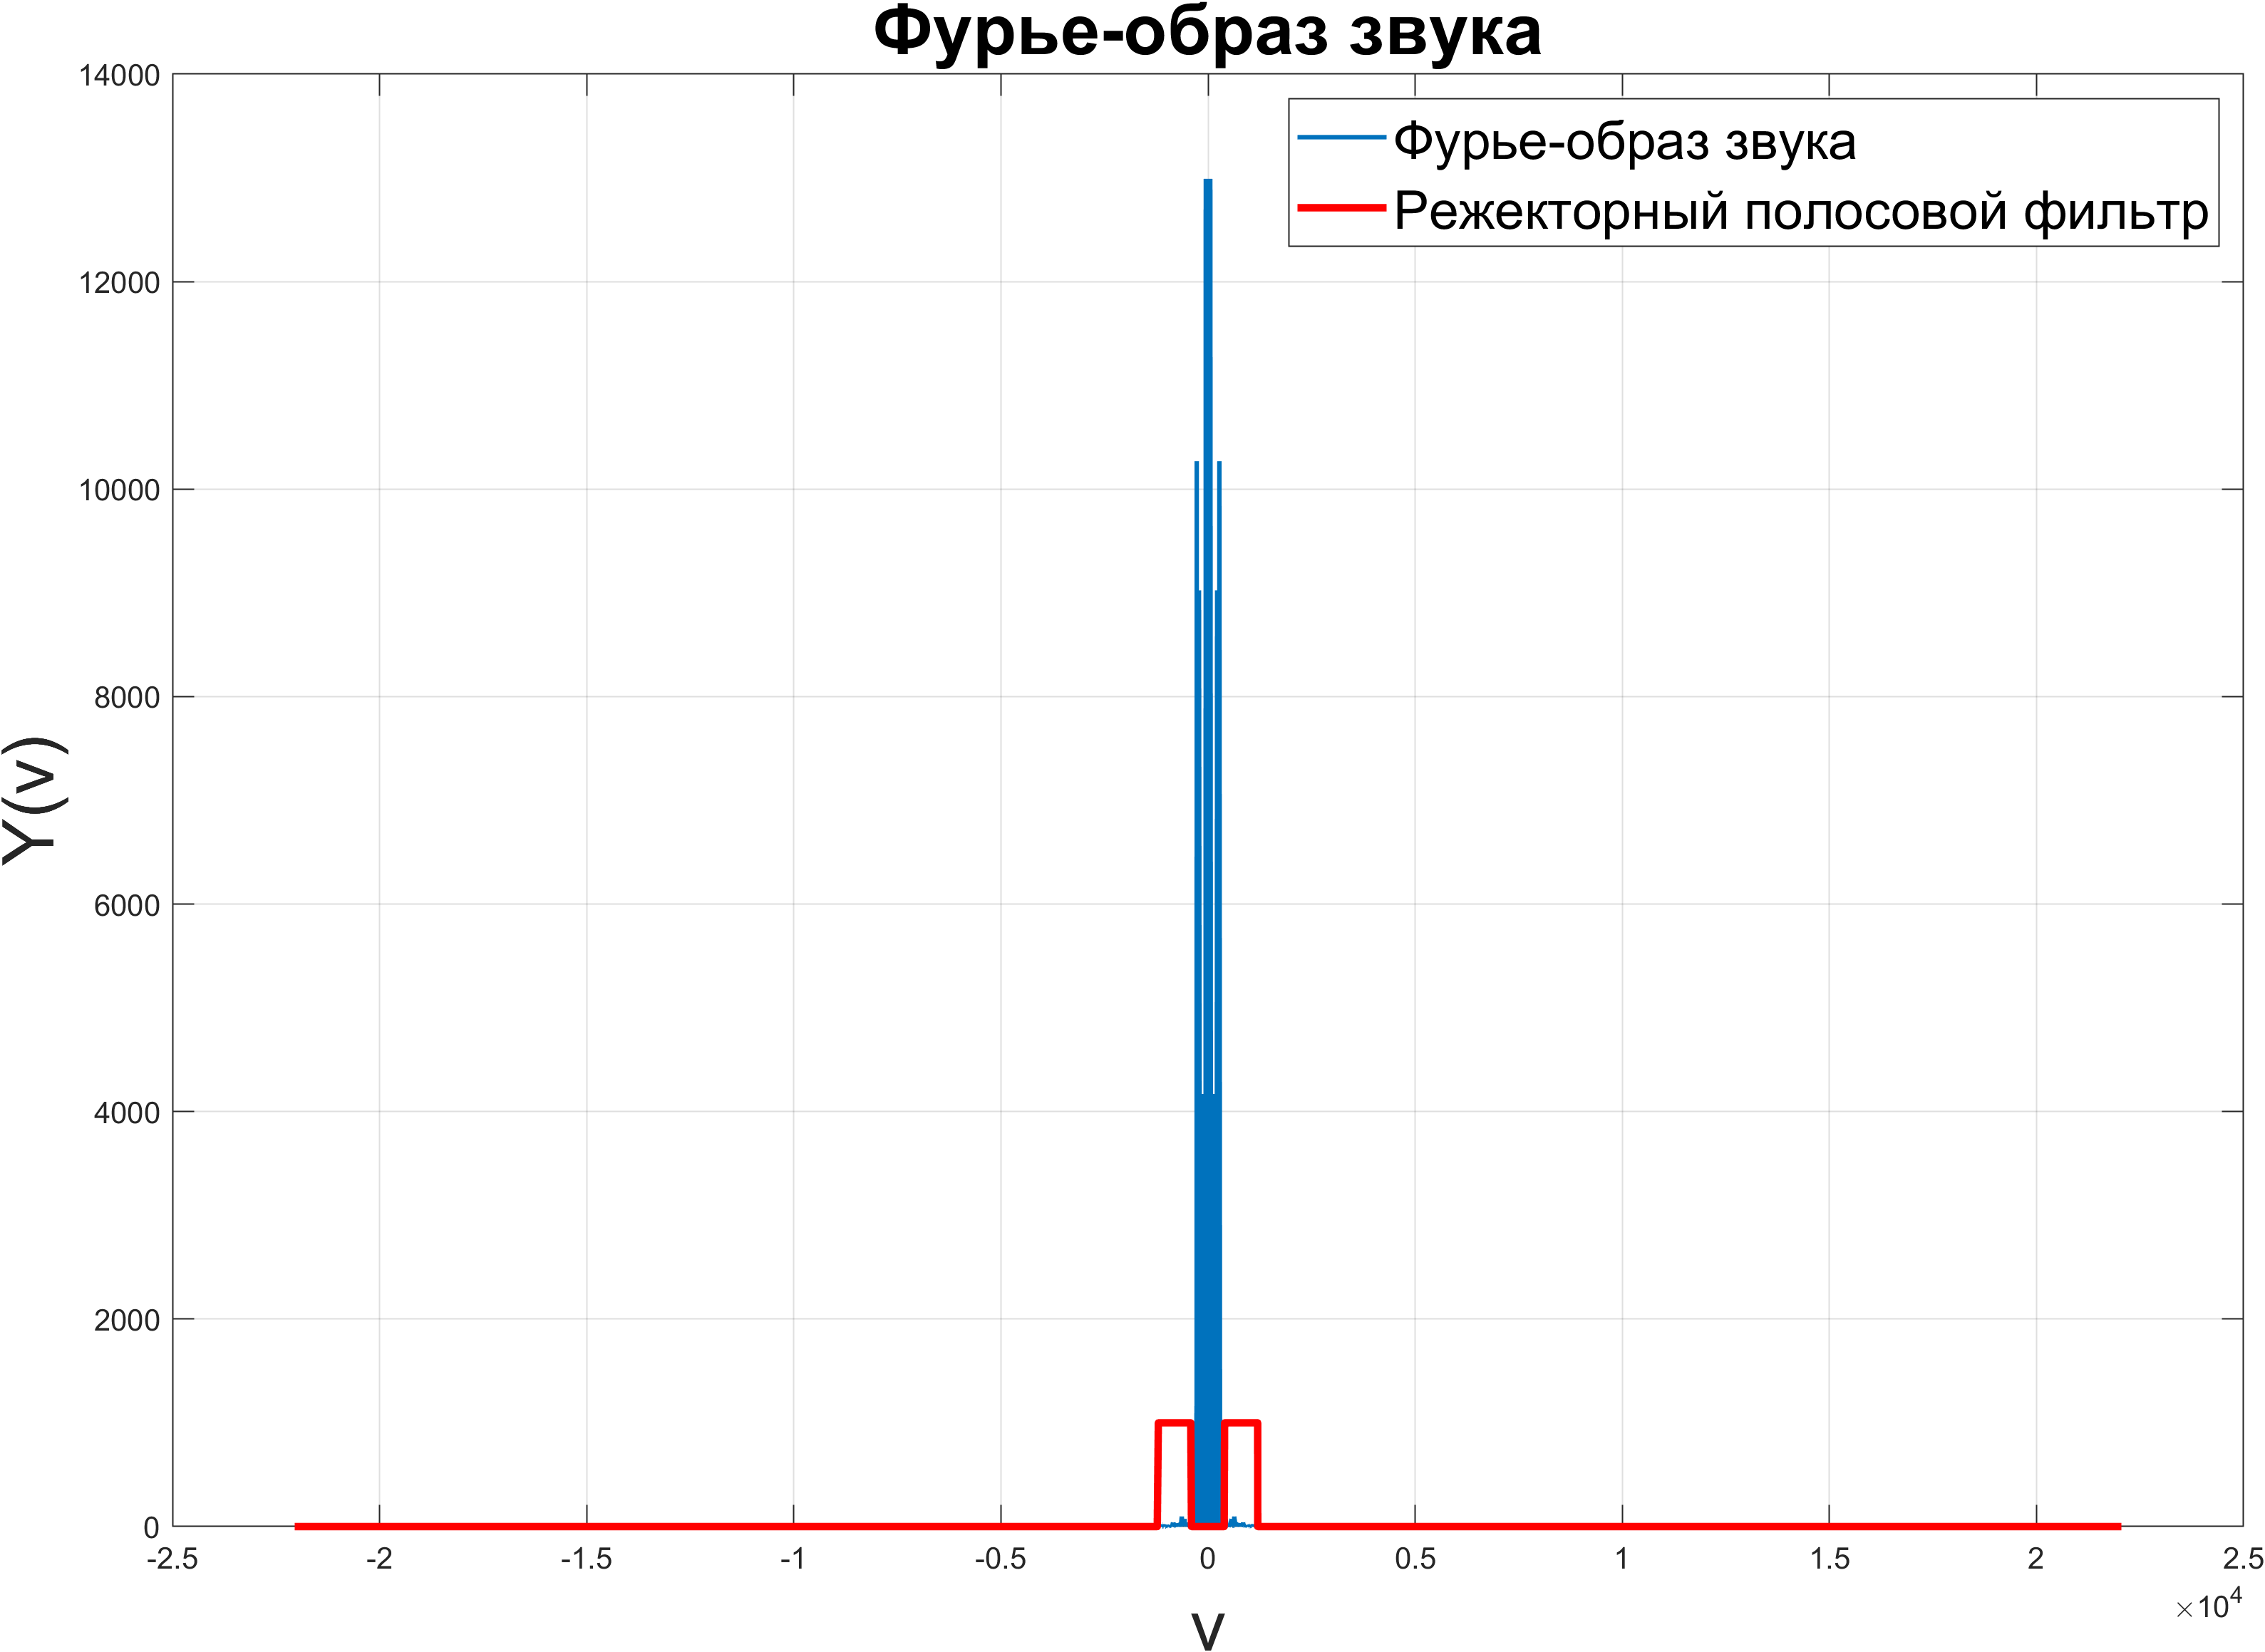
\includegraphics[width=1.0\linewidth]{images/fur_muha.png}
    \caption{Фурье-образ звука}
    \label{fig:noise}
\end{figure}
На этой картинке значения фильтра домножены на 1000, для наглядности. Диапозон фильтра \([-1000; -400] \cup [400; 1000]\). Фильтр отсёк все(или по крайней мере заметную часть) частоты, нехарактерные человеческому голосу, таким образом на записи остался лишь голос.
\begin{figure}[H]
    \centering
    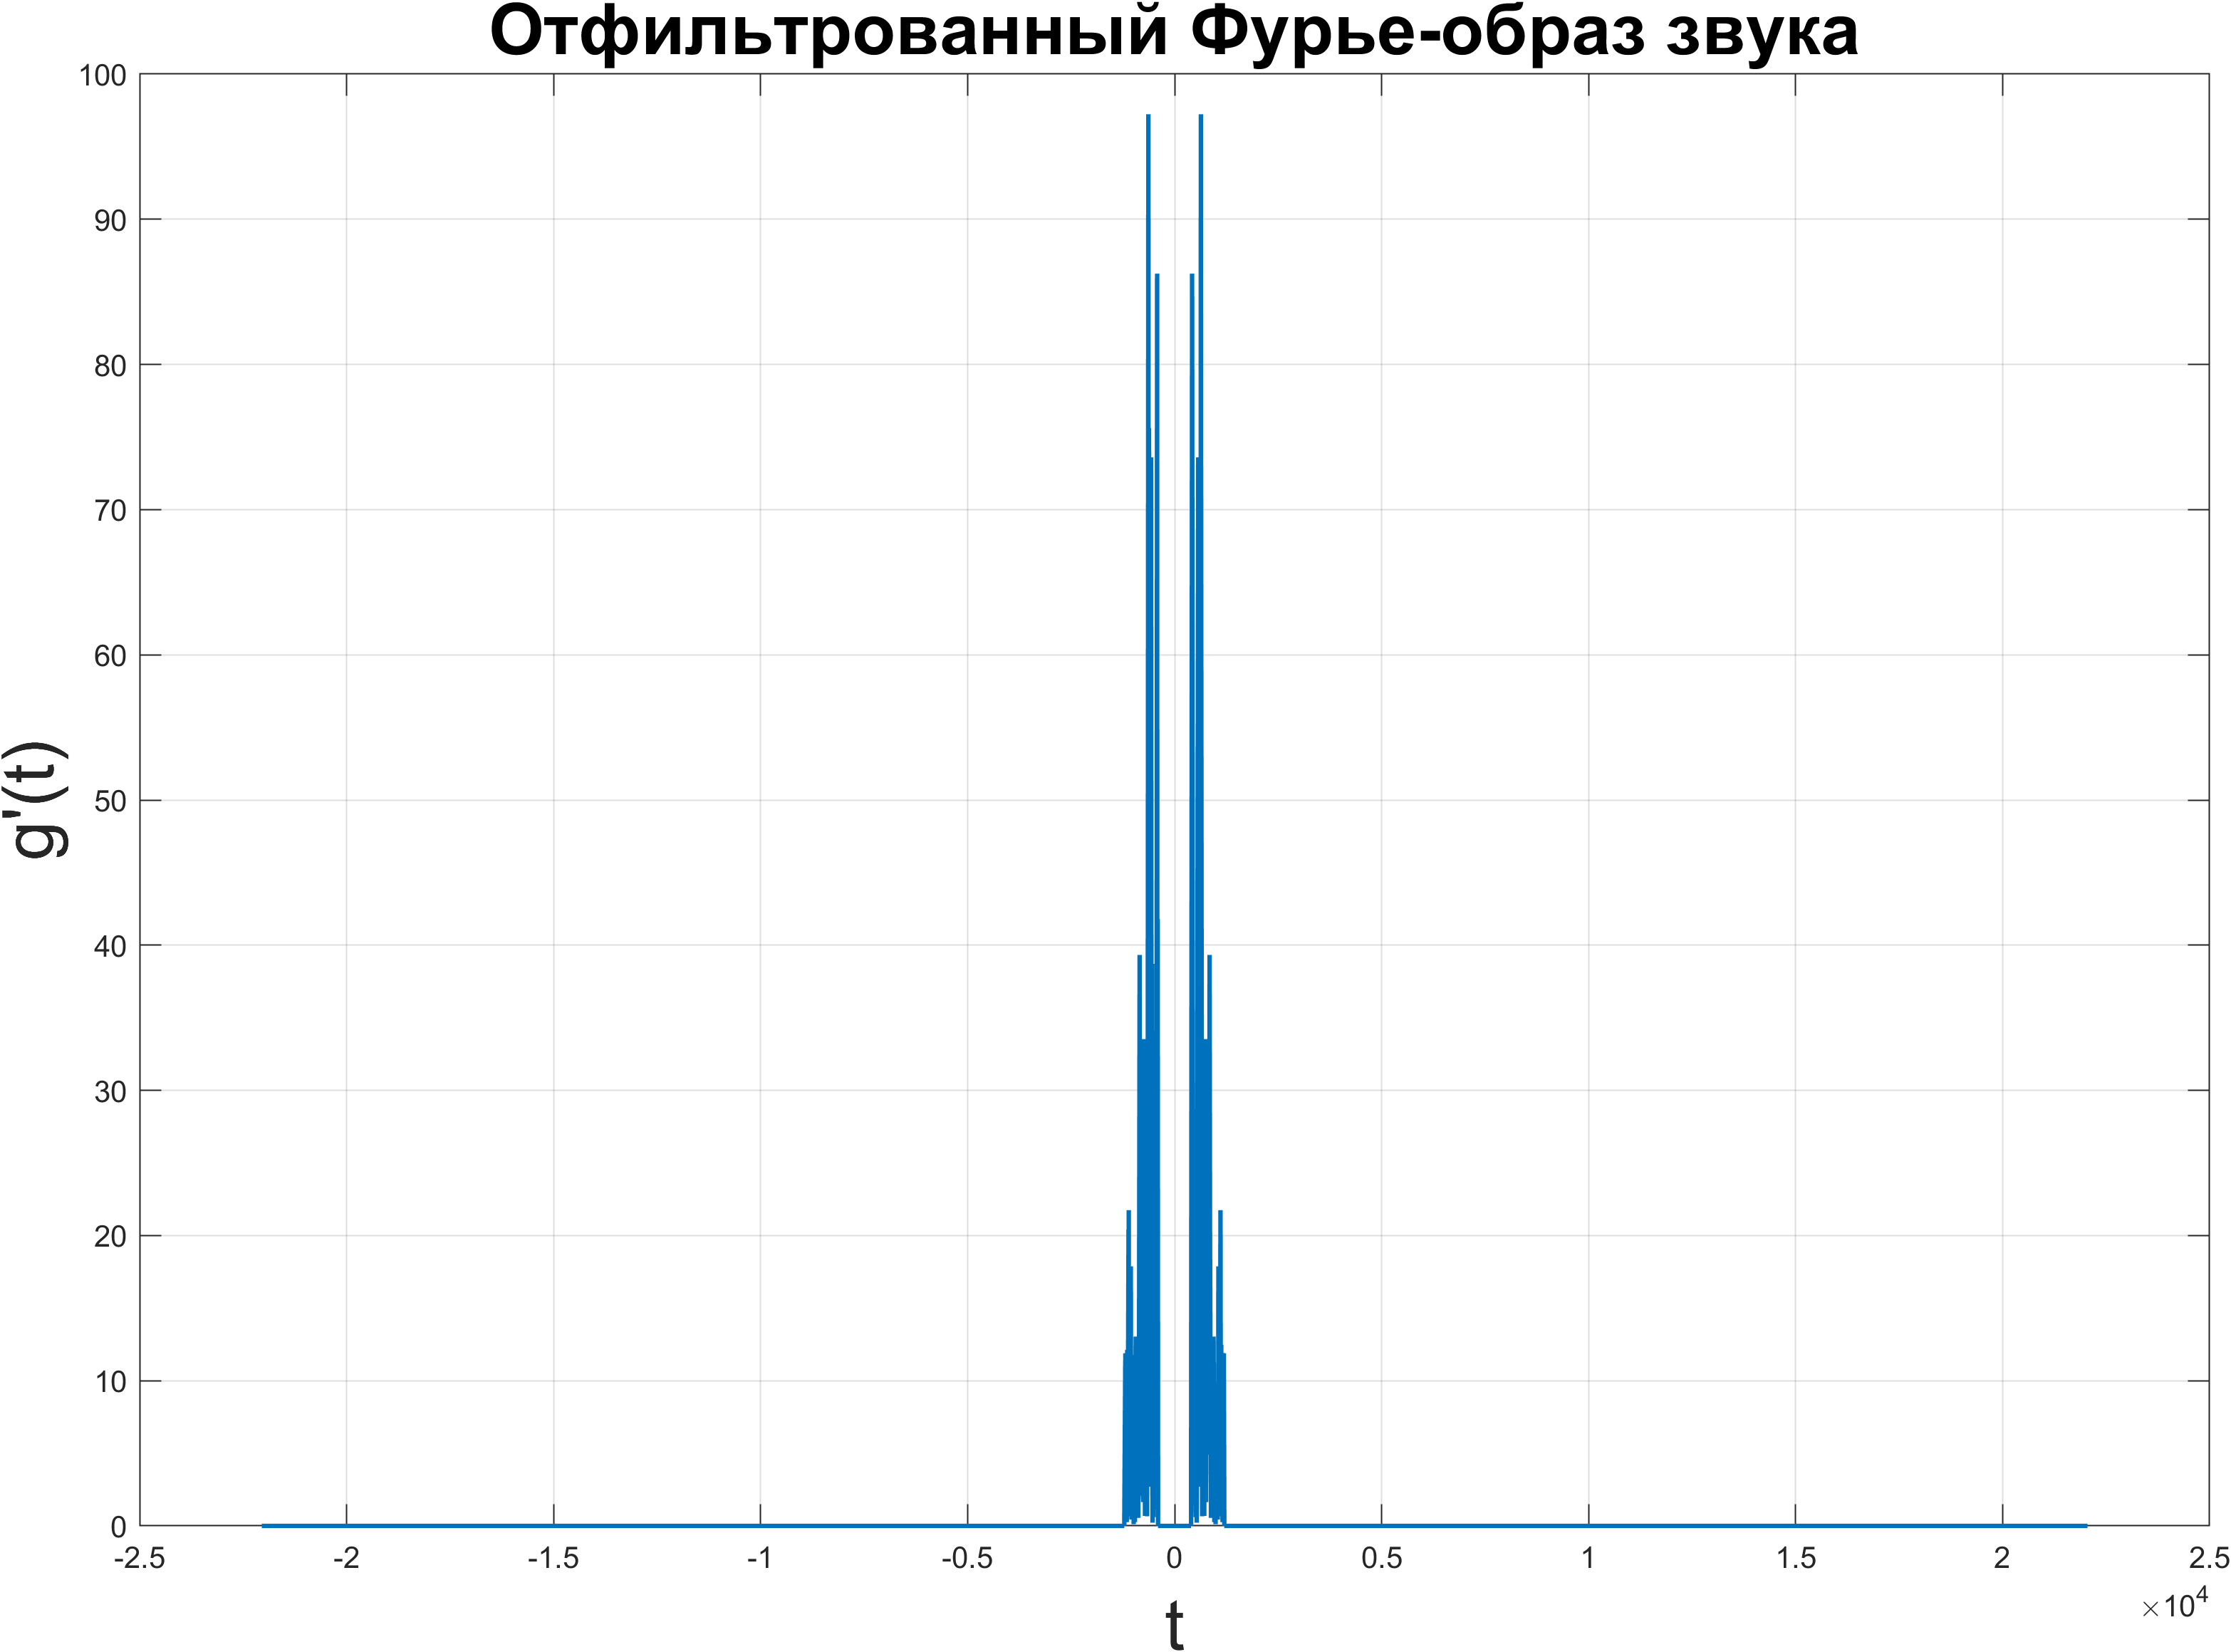
\includegraphics[width=1.0\linewidth]{images/filtered_fur_muha.png}
    \caption{Отфильтрованный Фурье-образ звука}
    \label{fig:noise}
\end{figure}
\begin{figure}[H]
    \centering
    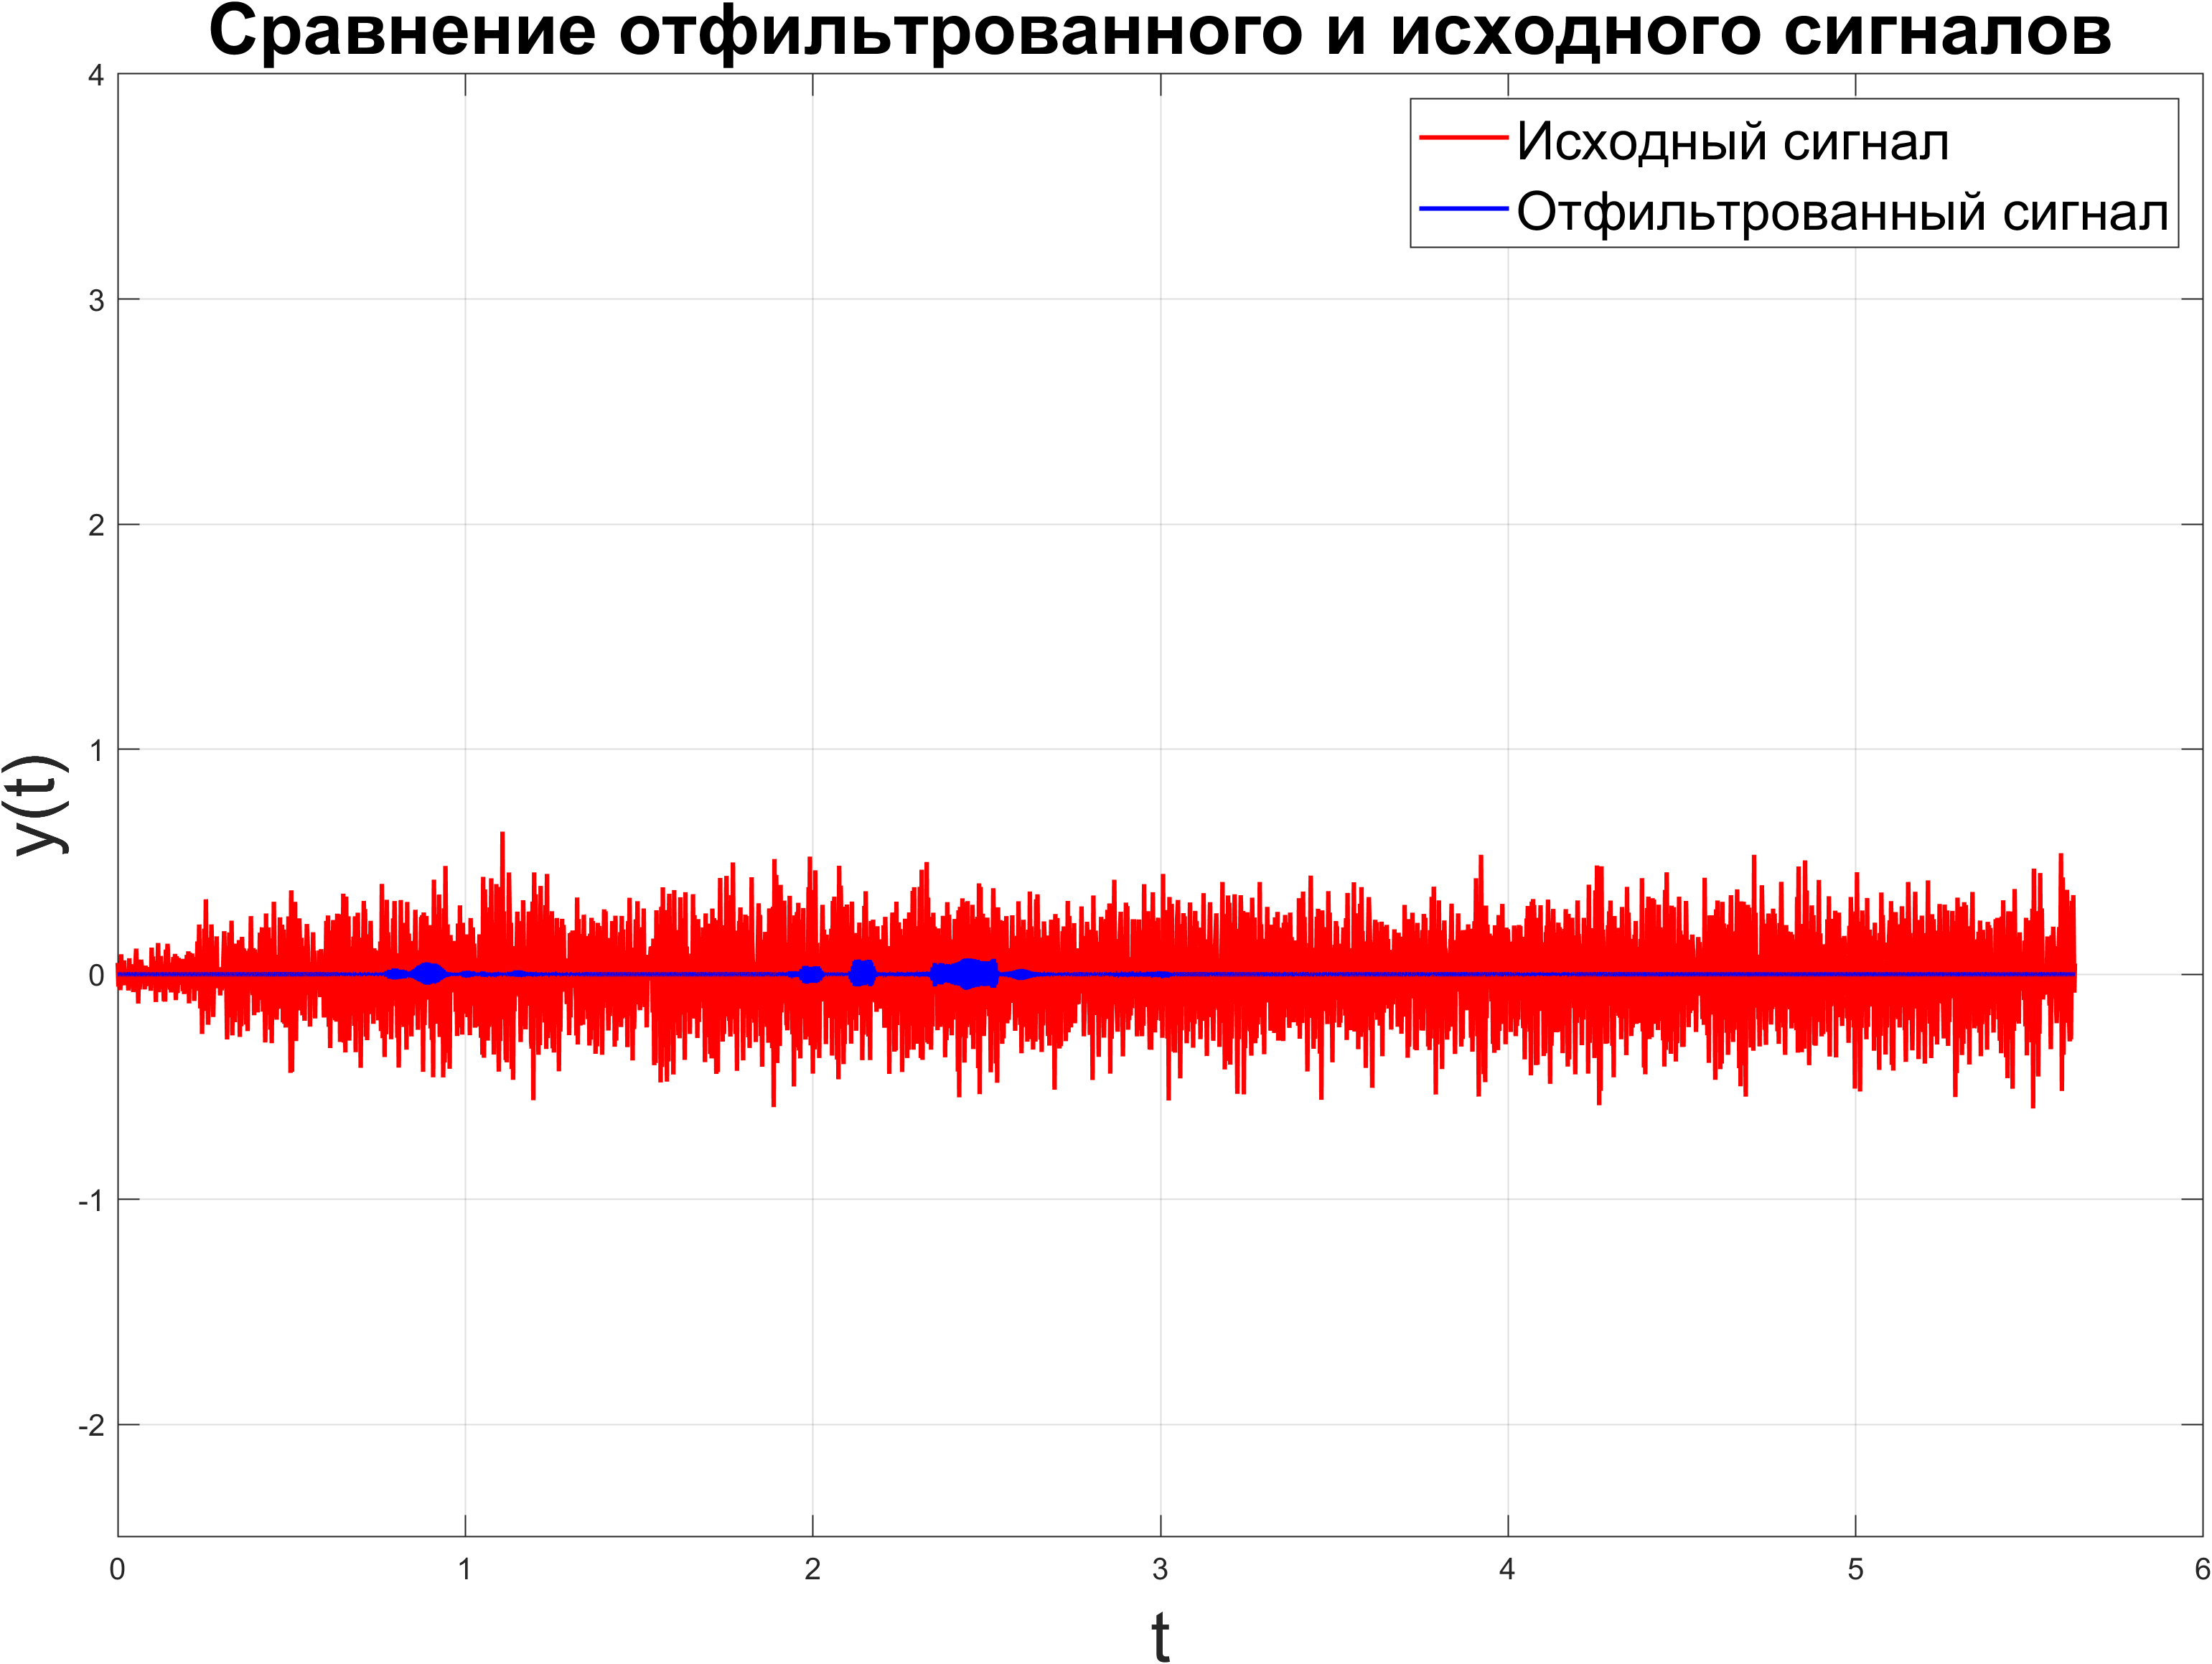
\includegraphics[width=1.0\linewidth]{images/filtered_muha.png}
    \caption{Исходный и отфильтрованный сигналы}
    \label{fig:noise}
\end{figure}

\end{document}
